\section{Relución de corto}
\begin{itemize}
    \item Población dependiente 
    \item Desempleados y no empleados
    \item Limites superiores e inferiores
    \item Efectos del salario mínimo
\end{itemize}

\section{Noticia: China planea cortar sus exportaciones de tieddas raras a EEUU}
\begin{itemize}
    \item Guerra comercial de EEUU y China
    \item Situación política con China en EEUU
    \item Los aranceles de EEUU son un 10\% adicional a los productos de China.
    \item Rare Earth metals, China no traerá a EEUU.
    \item Hay muchas regulaciónes en EEUU de tierras raras, en China no hay muchas regulaciónes del medio ambiente.
    \item En China es mas barato el proceso por la falta de regulaciones.
    \item China no tiene mucho poder de negociación en los diálogos entre EEUU y China.
\end{itemize}

\textbf{Discusión de la noticia}
\begin{itemize}
    \item Las estadísticas del Gobierno Chino no pueden ser fiables, se dicen decir estar contaminados.
    \item Discrepancia, en China es prohibido exportar de capital, no se pueden mover a otro país. Analogía de la puerta y el campo.
    \begin{itemize}
        \item Los chinos les combiene facturar de más para poder sacar el capital.
        \item El incentivo es a no facturar lo que es porque el gobierno chino prohibe la salida del capital.
        \item Sobrefacturación es un problema para las cifras.
    \end{itemize}
\end{itemize}


\section{Discusión de clase}
\begin{itemize}
    \item Las vacaciones son obligatorias, producto de los sindicatos y uniónes, \textbf{Nos preguntamos:} ¿curioso no?
    \item Parece que son los sindicatos los que han brindado eso, \textbf{el máximo que se le puede pagar a un trabajador es su productividad económica} que paternalista que las quotas de las personas deben pagar a los trabajadors como irtra, IGGS, etcétera.
    \item \emph{\textbf{Caso} ``AVI": quota obligatoria que parece ser que lo pagan los emprearios pero en realidad los paga el trabajador, los bonos y las quotas las paga el trabajador; la pregunta es cuánto produces y por cuánto te tengo que pagar; si se hace un bono 15 o cualquier quota extra absorbida que produce que el coste laboral aumenta lo paga el trabajador}
    \item Solamente cuando eres productivo puedes tener dependientes.
    \item Las leyes les valen a la economía, si se prohibe la gravedad no implica que la gravedad vaya a desaparecer. 
    \item Las leyes de Guatemala son increíblemente restrictivas.
    \item Desempleo friccional: las oportunidades que se abren y la gente las toma en el ámbito.
    \item Gente con salario de reserva muy alta es probable que estén sobre pagados.
    \item La ayuda social hace dependiente al trabajador y \textbf{sube} el salario de reserva de las personas.
    \item Guatemala es de los países que menos hace esto, esto es algo bueno. 
\end{itemize}

\section{Principles of economics - Carl Menger}
\begin{itemize}
    \item Bien y bien económico: \emph{\textbf{(Paréntesis:}Libros de sánscrito\textbf{)}}, \emph{\textbf{Definición de `bien":} es todo lo que se AUDIO 45.00}
    \item \emph{\textbf{Definición de ``Bien económico":} tiene que ser un bien que satisface necesidades humanas, pero tiene que ser escaso, es decri que algunas personas se van a quedar sin satisfacer la necesidad; ocurren dos cosas \textbf{lo economizas y lo intentas reproducir o multiplicar}.} \textbf{Nos preguntamos:} ¿Quién se queda con qué? \emph{(\textbf{Respuesta}:Los bienes libres son aquellos que no se economizan por ejemplo el aire, bienes semi-libres, quien se queda con el bien económico \textbf{los que lo valoran más}, este es un mecanismo de asignación.})
    \item Mecanismos de asignación: mercado, gobierno que raciona \emph{\textbf{Definición de ``racionamiento":} las cantidades existentes se dividen por el número de personas que lo demandan}, el que más lo valora.
    \item \textbf{\emph{(Ejemplo: el pedo, comportamiento económico para acudir el aire limpio, en ese momento el aire es un bien economico, porque se necesita economizar típico de un bien económico.)}}
    \item Bias de la prensa
    \item Los paises desarrollados tienden a aumentar su bosques, \textbf{Nos preguntamos:} ¿por qué?; la gente ya no usa leña para cocinar, la leña es ineficiente y además se considera esta forma de cocinar porque la gente es pobre.
    \item La sensibilidad ambiental que surge a partir de \$1,000 de renta per capita la gente empieza a demandar verde. Eso provoca que la oferta provea un bosque, un parque, etcétera. Esto se llama \textbf{curva de kuznetx Ambiental}
    \item La siguiente gráfica demuestra la destrucción ambiental respecto a la destrucción del medio ambiente. \emph{Citación:``El arbol como bien público", no se cuidan los bienes comunales, en lugar de decir no imprimas por que eso implica hacer papel de un árbol, decir: porfavor impriman para que yo pueda reforestar más.} 
    \begin{figure}[htbp]
        \centering
        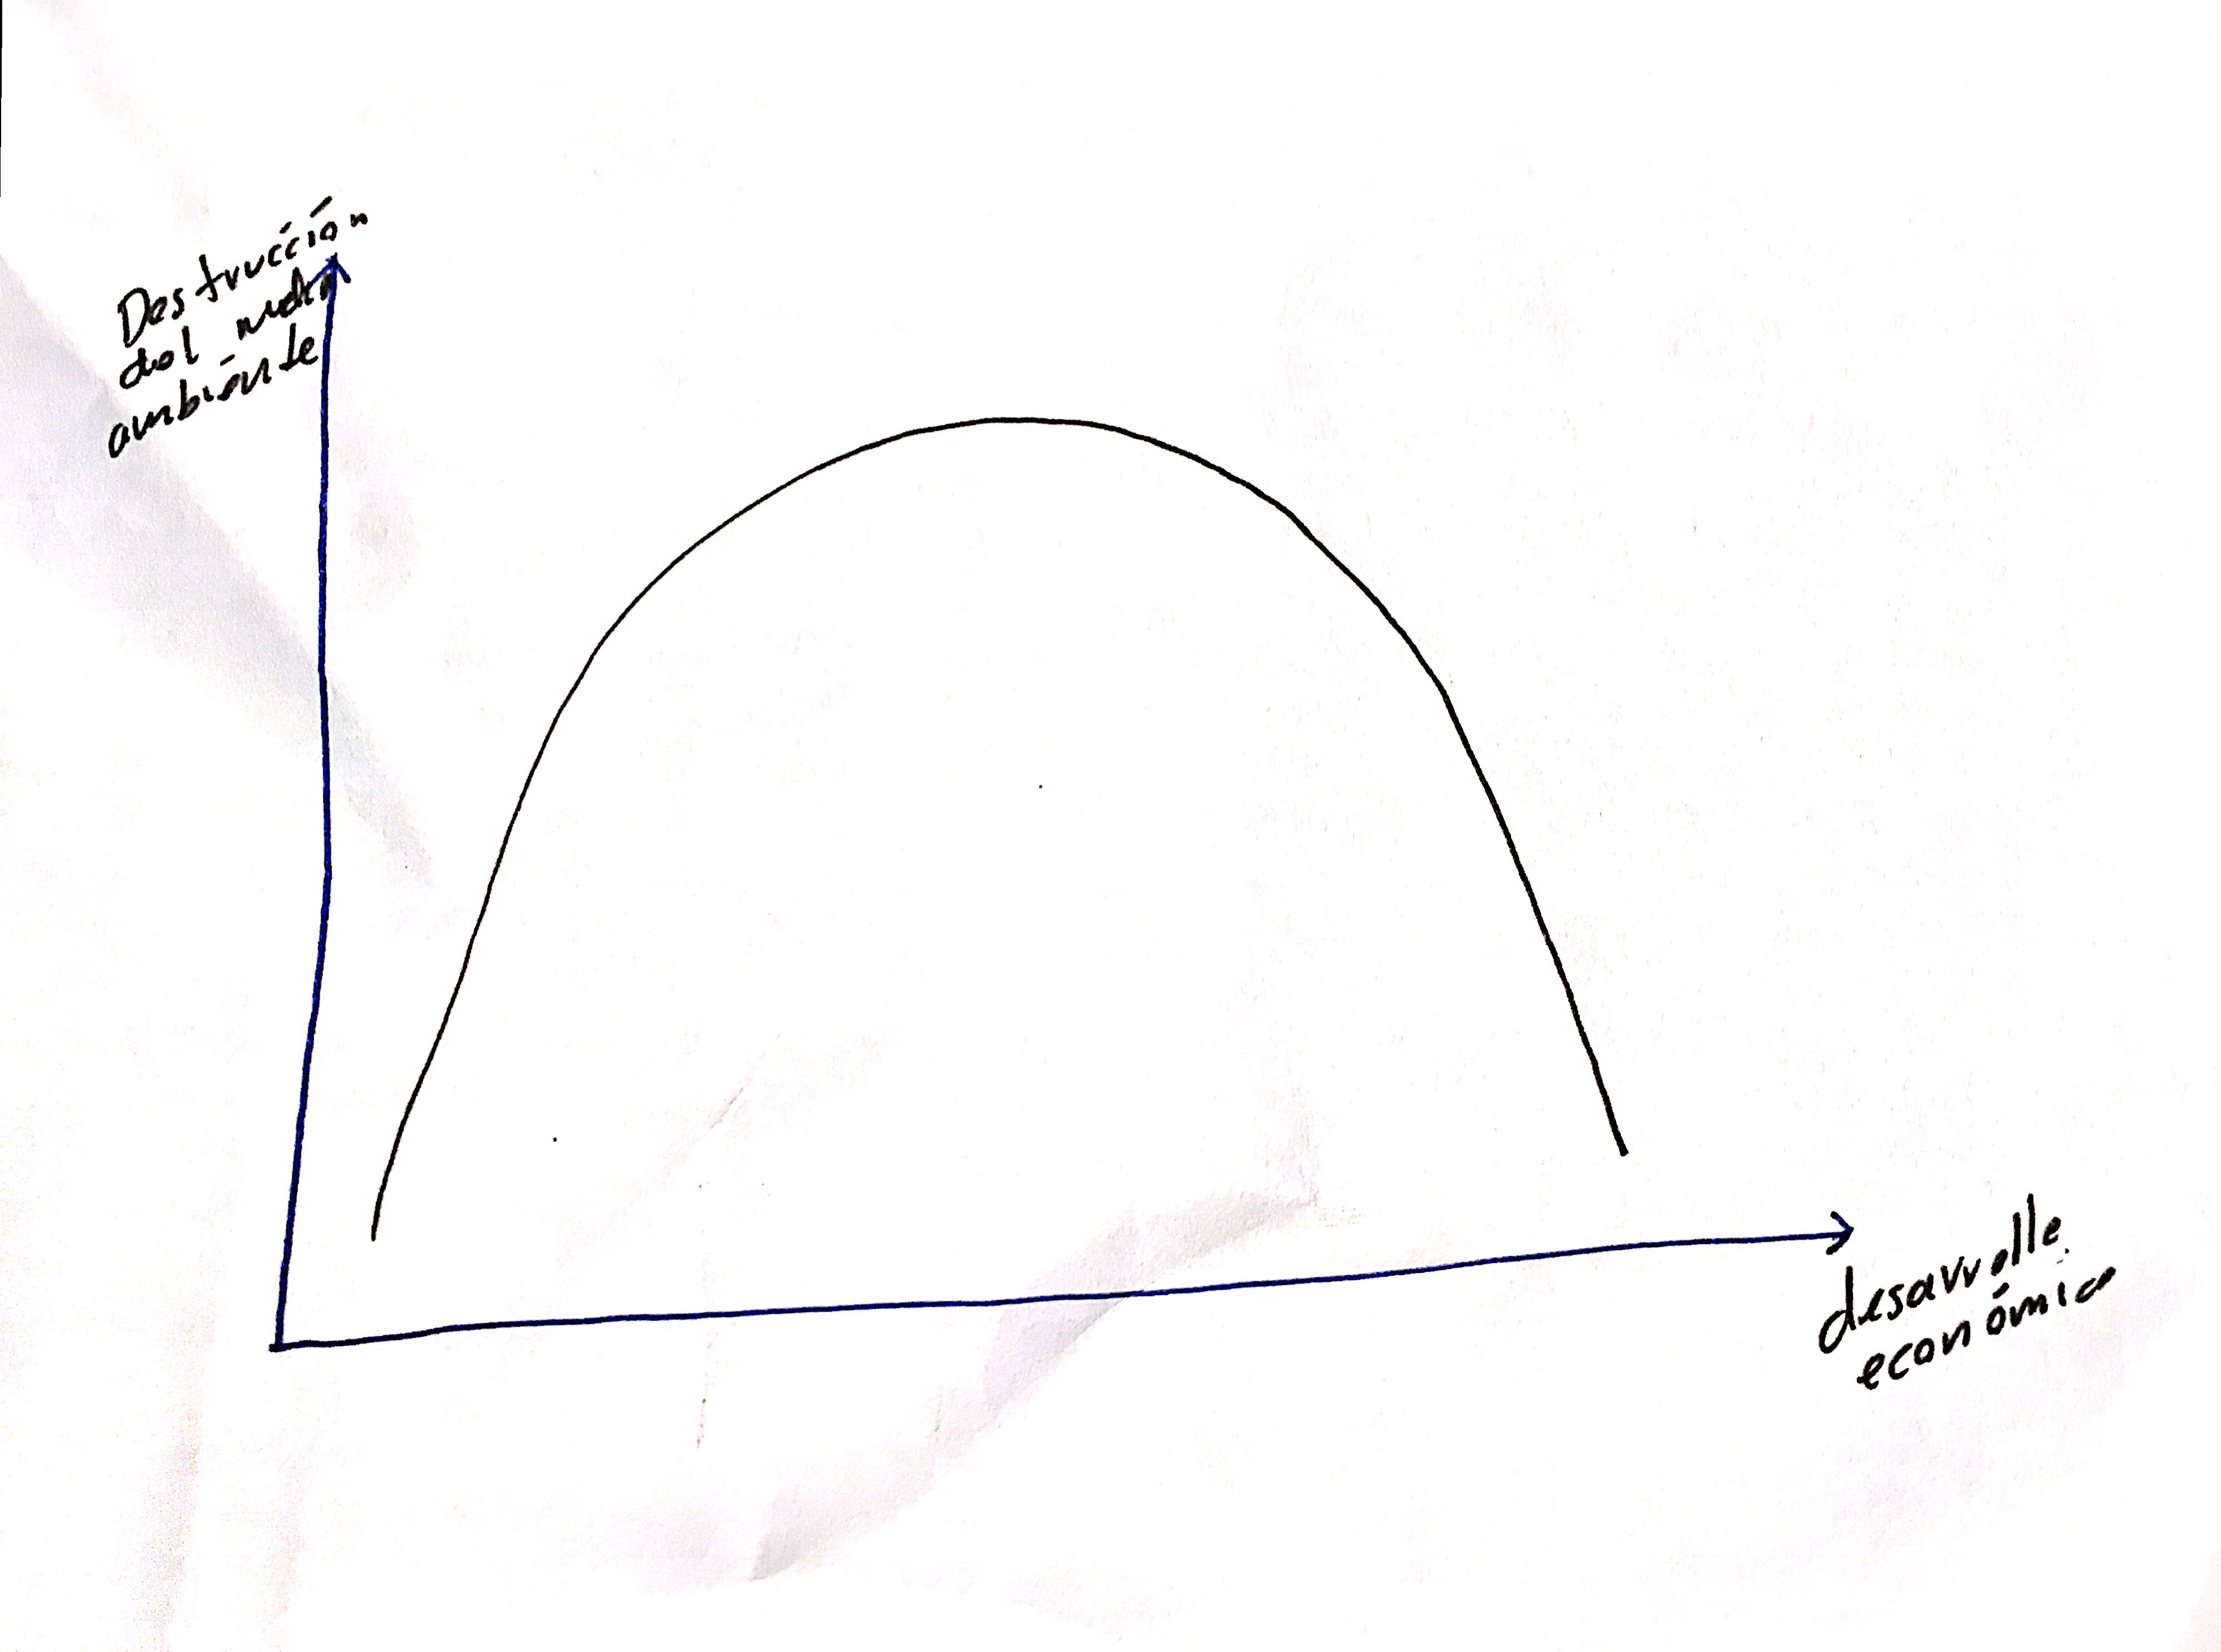
\includegraphics[width=6cm]{Classes/Images/2019-08-26-01.jpg}
        \caption{La destrucción ambiental respecto a la desigualdad de destrucción del medio ambiente}
        \label{}
    \end{figure} 

    
    \item Como una característica de un bien económico, es de la de querer multiplicarlo, mientras más se demanda el papel o los productos derivados de la desforestación más se oferta y más incentivo de querer multiplicar el bien económico que es escaso.
    \item En conclusión es mentira lo de las amazonas por la curva de Kuznets.


\end{itemize}
